\documentclass[11pt, a4paper,twocolumn]{jarticle}
\usepackage[dvipdfmx]{graphicx}
\usepackage{listings,jlisting}

\begin{document}
%=============================================================
\section{Measurement of current-voltage characteristics of thermistor (metal-oxide semiconductor) and mechanical pencil lead(carbon)($5^{th} day$)}

\subsection{Purpose}
サーミスターとシャープペンシルの芯の電気抵抗の温度依存性を学習する.
\subsection{Procedure}
今回はサーミスター(103AT-11)とシャープペンシルの芯(H,2B)について測定をおこなう.
まず前回同様に図\ref{fig:29}のように装置を組み立てて四段階に温度を変えながら測定を行った後,それぞれの抵抗値を電流電圧測定値の傾きを最小二乗法によって求め温度依存性を考察する.

\begin{figure}[htbp]
 \begin{center}
  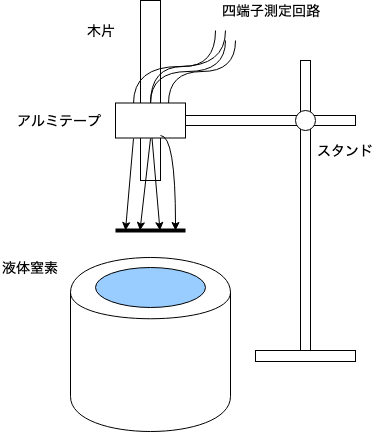
\includegraphics[width=0.8\linewidth]{fig29.png}
 \end{center}
 \caption{温度依存性の実験装置}
 \label{fig:29}
\end{figure}

\subsection{Result}
測定の結果温度と抵抗値の関係をプロットすると以下のようなグラフが得られた.
シャーペンの芯はどちらの芯も同じ温度依存性を示した.
またサーミスターに関しては温度依存性を示さなかった.

\begin{figure}[htbp]
 \begin{center}
  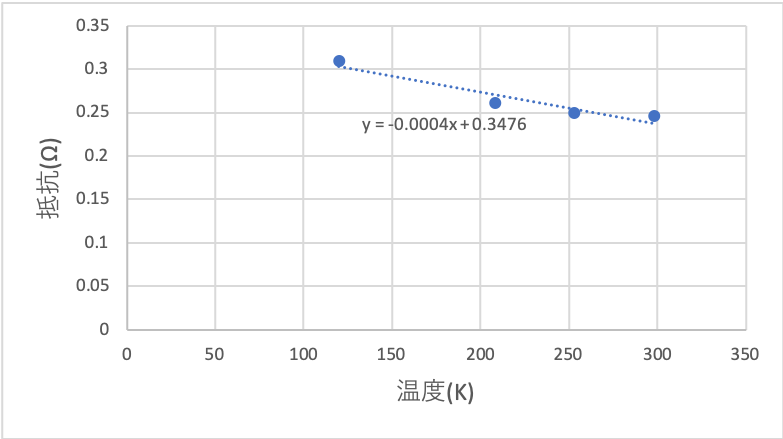
\includegraphics[width=0.8\linewidth]{fig33.png}
 \end{center}
 \caption{カーボン2Bの温度依存}
 \label{fig:33}
\end{figure}

\begin{figure}[htbp]
 \begin{center}
  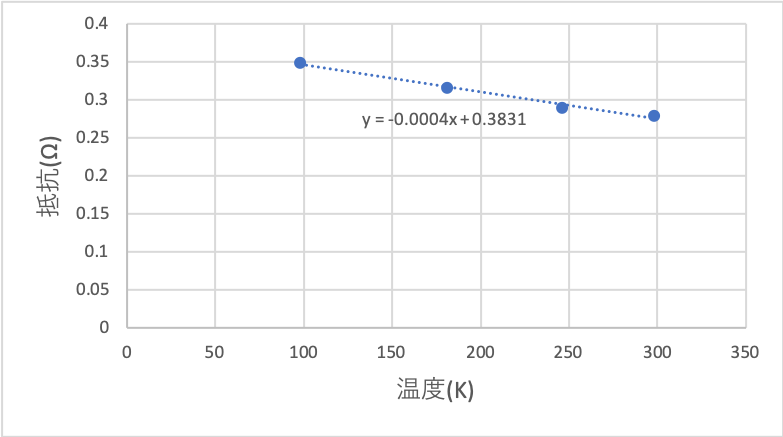
\includegraphics[width=0.8\linewidth]{fig34.png}
 \end{center}
 \caption{カーボンHの温度依存}
 \label{fig:34}
\end{figure}

\begin{figure}[htbp]
 \begin{center}
  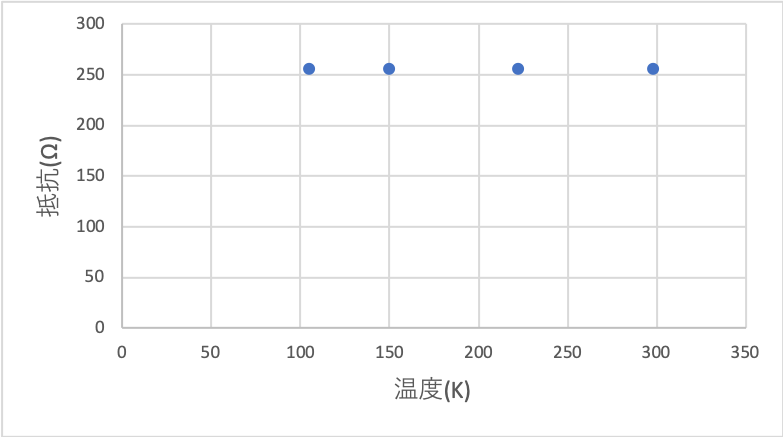
\includegraphics[width=0.8\linewidth]{fig35.png}
 \end{center}
 \caption{サーミスター(103AT-11)の温度依存}
 \label{fig:35}
\end{figure}

\subsection{Discussion}
前回の実験において室温でのシャープペンシルの芯は硬さに関わらず同じ抵抗値を示したのでシャーペンの芯の抵抗特性は硬度に依存しないと考えられたが,今回の実験でもこの二つの硬さにおける測定値に有意な差は観測てできなかったので硬さによってシャープペンシルの芯の構造は変わらないと考えられる.
サーミスターの測定結果より今回の実験ではサーミスターの温度特性を観測できなかったので実験の操作手順をミスしてしまった可能性が考えられる.
もしくはサーミスターの抵抗変化が高温で起こることなどが考えられる.

また今回は前回の金属試料の温度特性と異なり温度が高くなるにつれて抵抗率が低くった原因について考察する.
エネルギーバンド図において非金属の半導体のバンド図は図\ref{fig:37}のようになる.
このバンド図において電子の多くは価電子帯に存在しており伝導体に存在する電子は少量と考えることができる.
温度が上がることにより励起される価電子帯の電子がエネルギーギャップEgを超えることにより伝導帯に存在する電子が増え,結果として抵抗率が小さくなっていくと考えられる.

\begin{figure}[htbp]
 \begin{center}
  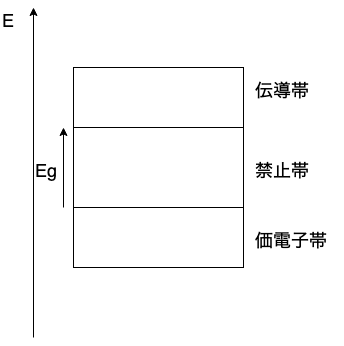
\includegraphics[width=0.8\linewidth]{fig38.png}
 \end{center}
 \caption{半導体のバンド図}
 \label{fig:38}
\end{figure}


%=============================================================
\newpage
\end{document}
